\section{MOOC overview}
\label{sec:mooc_overview}

This section consists of an overview about a massive open online course (MOOC).

The Mooc (Massive Open Online Courses) are open online courses designed for distance learning that involve a large number of users.
The authoritative site www.moocs.co calls them “free non-degree online courses with open enrollment unlimited global to anyone who desires to learn, and regardless of their current educational level”. \cite{mooc_def}

The first Massive Open Course was created by Professor O'Donnell, University of Pennsylvania, but the term MOOC actually was created in 2008 by Professor Cormier, University of Prince Edward Island.


Compared to the attempts of e-learning made in the past, this time there was a quantum leap, not only because promoting them are some of the most prestigious universities in the world (from the MIT in Boston at Harvard, through Stanford and Berkeley) but also because it has finally gone beyond the usual video-lessons, to really embrace interactivity between teachers and students, including peer-to-peer interactivity as well.

E-learning, therefore, means not only learning through digital media, but a new digital way of relating to study and education.
Its features are:
\begin{itemize}
\item Modularity: You can select courses and lectures on topics of your interest;
\item Flexibility: You can take lessons at any place and at any time of the day;
\item Collaboration: You can relate with other students in a constructive way, exchanging opinions and materials;
\item Continuity: You can study and inform continuously and deepen your passions, without putting an end to your training path.
\end{itemize}

In 2012 the MOOC were about 100 and almost 700 in 2013 (an average of 2 new MOOC offered every day). In total more than 1200 courses announced.


\begin{figure}[htb] %  figure placement: here, top, bottom
 \centering
 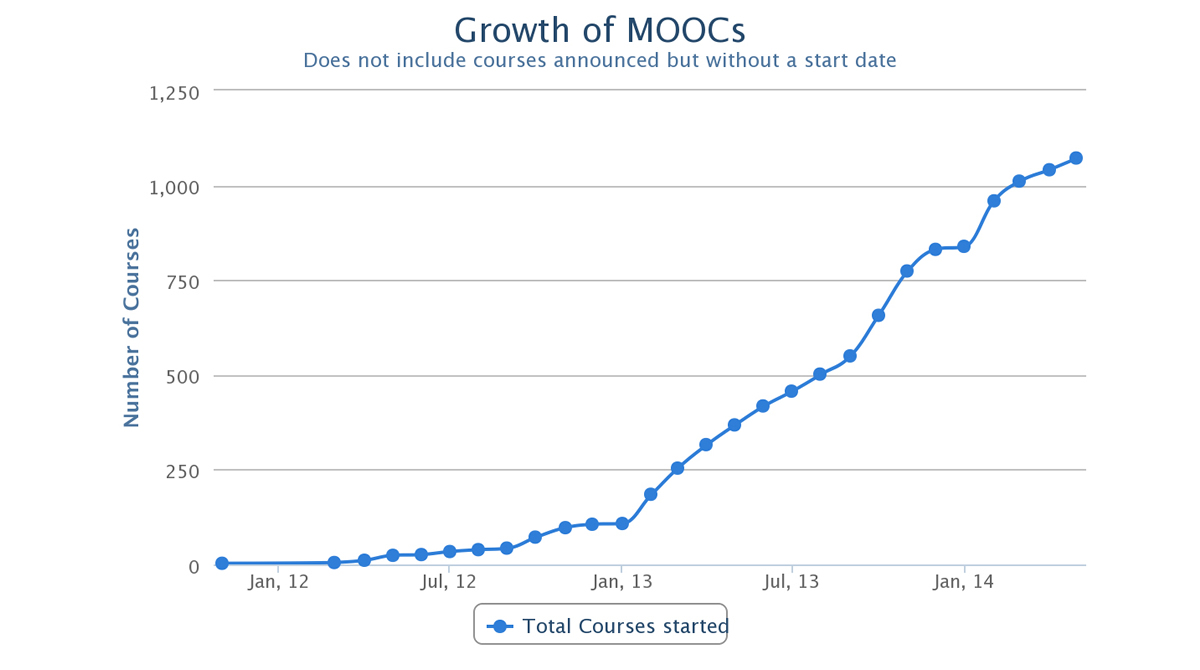
\includegraphics[width=0.8\linewidth]{images/chapter1/mooc.jpg}\hfill
 \caption[Growth of Mooc]{Growth of Mooc}
 \label{fig:fourV}
\end{figure}


Early MOOCs often emphasized open-access features, but some later MOOCs use closed licenses for their course materials while maintaining free access for students.\cite{mooc_wiki}

Although not replacing a traditional degree program, the MOOC offers valid proof of good participation to students that may be used in the Curriculum Vitae. While the courses are absolutely free, often to secure a certificate of attendance it is required to pay a fee. The amount of the fee varies according to the organizer.


It took some time before everyone would realize the enormous potential of MOOC, but according to The New York Times, 2012 became “the year of the MOOC”\cite{pappano2012year} and a large number of sites like Udemy, and Coursera EDX joined the market of training and development.

In the first platforms MOOC courses were held by the teachers of the universities, but this trend has changed in recent years and has seen the rise of platforms where anyone can create their own course.

Some platforms were born like Udemy which are similar to MOOCs but these work outside the university system and emphasize individual self-paced lessons.

In May 2013 the Udacity announced the first entirely MOOC-based master's degree, a collaboration between Udacity, AT\&T and the Georgia Institute of Technology, costing \$7,000, a fraction of its normal tuition.\cite{mooc_wiki}

